\documentclass[abstract=on,a4paper]{scrreprt}
\usepackage[utf8]{inputenc}
\usepackage{float}

\usepackage{natbib}
\usepackage{graphicx}
\usepackage{subfig}
\usepackage{tikz}
\usepackage{pgfplots}
\usepackage{todonotes}
\pgfplotsset{compat=1.12}
\usepackage{textcomp}
\usepackage[toc,page]{appendix}
\usepackage{hyperref}
\usepackage{pdfpages} %added by Ali for pdf vedlegg
\usepackage{comment}

\usepackage{geometry}
 \geometry{
 a4paper,
 total={170mm,257mm},
 left=20mm,
 top=20mm,
 }
 
 
%-------------------------------------------
\newcommand\Block[2]{%
\setlength\fboxsep{0pt}\setlength\fboxrule{0.1pt}% delete
\fbox{% delete
\parbox[c][.5\textheight][t]{0.3\textwidth}
{#1\par #2}
%
  }% delete
}
%--------------------------------------------

\renewcommand{\figurename}{Figur}
\renewcommand{\tablename}{Tabell}
\renewcommand{\contentsname}{Innholdsfortegnelse}
\renewcommand\appendixpagename{Appendiks}
\renewcommand{\bibname}{Kilder}
% Edit the meta.tex file to change title, group number and author names
% Fill in the report title, group number and student names here
\newcommand{\mytitle}{Prosessrapport}
\newcommand{\mygroupnumber}{2}
\newcommand{\myauthor}{\\Ali Aljumaili (772170) \\ Anders Gildberg (750003) \\ Håkon Prestegård (750419) \\ Jonas Lien (741392) \\ Lars Kambe Fjæra (748650)}


\title{\mytitle}
\author{\myauthor}
\date{\today}




\begin{document}
% The title page, edit if you want to customize it
\begin{titlepage}

\includegraphics[height=1.5cm]{images/ntnu_logo.pdf}\\[1cm]   
\begin{center}

 
% Upper part of the page
~\\[1.5cm]

\textsc{\Large TDT4856 IT-styring av moderne lastebiler}\\[0.5cm]

% Set the title of the Document between two horizontal lines
\hrule ~\\[0.2cm]
{\huge \bfseries \mytitle}\\[0.4cm]		% print the title of the document
\hrule ~\\[1.5cm]

% Additional Information about the document
\begin{minipage}{0.4\textwidth}
    \centering
	\large
		\emph{Group \mygroupnumber:}
		\myauthor
\end{minipage}

\vfill

% Bottom of the page
{\large 3. Mai 2017}

\end{center}
\end{titlepage}

\newpage
\tableofcontents{}

% Main matter - edit corresponding file under content/ to change
\chapter{Introduksjon}


Denne rapporten tar for seg gruppemedlemmenes erfaringer, forkunnskaper og forventinger til faget vil bli presentert, samt tre forskjellige samarbeids-caser som har oppstått under arbeid sammen dette semesteret. Det skal diskuteres og reflekteres over disse casene slik at læringsutbytte blir størst mulig. Rapporten konkluderer med tre erfaringer hvert medlem tar med seg videre, samt tre felles gruppeerfaringer.\\

Vi ønsker å takke faglærer Svein-Olaf "Sophus" Hvasshovd for faglig støtte og input gjennom semesteret, Terje Moen ved Sintef Teknologi og Samfunn og Arvid Aakre ved institutt for Bygg og Miljøteknikk for gode samtaler og innspill, samt læringsassistentene Martine Gran og Julian Vollen for veiledning og fasilitering. Vi ønsker også å takke Nordic Semiconductor som bidro med gratis utviklingskort, Omega Verksted for lån av fasiliter og Hackerspace NTNU for lån av byggesett.



\chapter{Presentasjon av medlemene}

\begin{figure}[h]
    \centering
    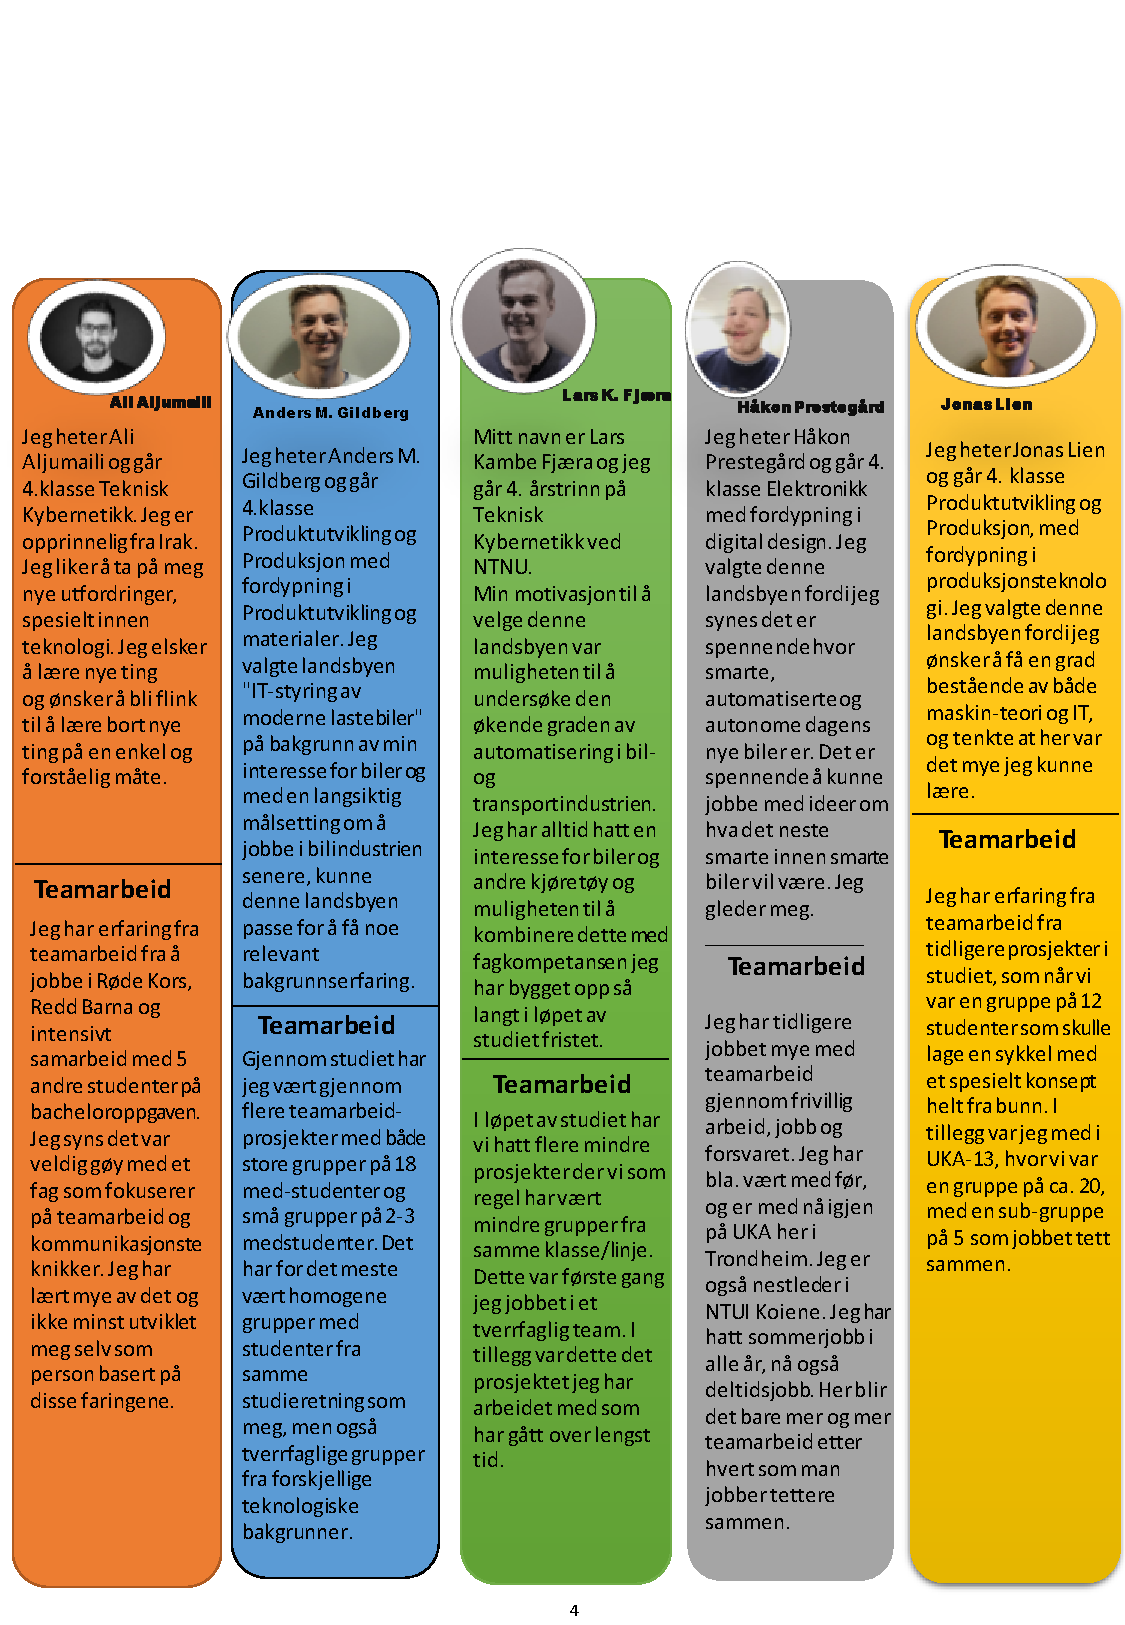
\includepdf[pages=1]{vedlegg/Medlemmer2.pdf}
    \label{vedlegg:presentasjon}
6\end{figure}\newpage





\chapter{Utvalgte situasjoner i prosjektperioden}

\section{Case 1 - En krangel mellom Håkon og Ali}

\subsection{Situasjon}


Klokka nærmer seg 15.30 og alle gruppemedlemmer kjenner at det har vært en lang og tung dag. Vi har jobbet iherdig gjennom dagen. Første halvdel gikk til prosjektoppgaven mens etter lunsj ble satt av tid til å diskutere vårt siste case. Det ble diskutert i nærmere èn og en halv time rundt temaet Alis forsentkomminger. Her kom det fram at gruppemedlemmene hadde forskjellige holdninger til å møte til avtalt tid. Det var en meget konstruktiv diskusjon med mange forskjellige synsvinkler og meninger. Her tenkte vi at vi virkelig hadde noe å skrive om, som kunne reflektere forskjellene mellom gruppemedlemmene. Vi var fornøyde og ble enige om å ta en kort pause, for så å gjenoppta diskusjonen. Jonas går en tur på toalettet, Anders går for å hente seg litt vann og Ali benytter pausen på å fullføre noe på datamaskinen. I det pausen er over og Jonas og Anders er kommet tilbake, blir Ali oppringt på telefonen. Han ser på telefonen og lurer på hvem det er som ringer. Han svarer ikke på telefonen og Håkon initierer gjenopptagelsen av diskusjonen vi skulle ha etter pausen. I det Håkon begynner å prate og ser seg rundt bordet for å fange øyekontakt med gruppemedlemmene, ser han at Ali sitter og tekster på telefonen.\\

\textit{"Ali, nå må du legge ned den telefonen og følge med! Samma om det er for en sommerjobb eller et annet fag, vi har blitt enige om at når vi diskuterer sammen så skal alle følge med."}{--Håkon}\\

Det blir med en gang stille i gruppen og Ali sine øyne spretter opp. Det går et sekund eller to før Ali helt får med seg hva som har skjedd. Jonas, Anders og Lars sitter med hodet lett presset bak, overrasket over situasjonen. Håkon virker passe irritert, og ønsker at gruppa skal følge det vi har sagt tidligere om at alle skal følge med når gruppa i felleskap diskuterer.\\

\textit{"Håkon, nå må du roe deg ned. Nå må du seriøst roe deg ned."}{--Ali}\\

Jonas bemerker seg at situasjonen begynner å gå opp for Ali, og synes han ser en irritasjon bygge seg opp i Ali etterhvert som han får tenkt litt på hva som har skjedd. Anders er redd for at situasjonen skal eskalere, og at det framtidige samarbeidet i gruppen står i fare. Anders legger spesielt merke til at stemmebruken og temperaturen er litt høyere enn hva han er komfortabel med.\\

\textit{"Når vi har blitt enige om at alle skal følge med når noen snakker, så syns jeg vi skal følge det, uansett hva det er"}{--Håkon}\\

\textit{"Noen prøvde å ringe meg, og jeg skulle bare svare og si at jeg var opptatt, og at jeg skulle ringe tilb... jeg behøver ikke å forklare meg for deg på denne måten for faen"}{--Ali}\\

Ali kaster oppgitt fra seg pennen han holder i hånden og ser ned i bordet og rundt i rommet med frustrasjon. Håkon prøver å forklare hvorfor han sa det han sa, og stod fortsatt for det han mente. Ali var fortsatt meget provosert og hintet til at dersom Håkon ikke sluttet å snakke, så ville han få en mobiltelefon servert i skallen. Lars, Anders og Jonas tenkte at det nå var lurt å ta en liten pause til for å roe seg ned. Deretter kunne vi så skrive ned situasjonen for å ta den opp og diskutere hva som hadde skjedd når ting kjølte seg litt ned.

\newpage

\subsection{Refleksjoner}

Sett tilbake på denne hendelsen, er det mange ting man kan spørre seg om hva som kunne blitt gjort annerledes eller bedre for å unngå en slik direkte konfrontasjon. Skjedde dette spontant, eller var det en reaksjon på noe som hadde bygget seg opp over lengre tid? Uken etter denne hendelsen tok vi opp temaet på nytt og snakket gjennom det i en mer nøytral og reflekterende forstand. Denne uka var Lars borte, men resten av gruppa satt en god halvtime og diskuterte hvorfor de trodde hendelsen utspilte seg som den gjorde. Vi startet med å ta runden rundt bordet og la hver person forklare hva de syntes om situasjonen.\\

Det startet med Anders og Jonas sine gjenfortellinger av situasjonen, som var ganske like. Anders mente han opplevde at Håkon kjeftet på Ali i måten han uttalte seg på og poengterte at han selv ikke ville likt å bli snakket til å den måten. Han hadde forståelse for at Ali ble provosert og reagerte på måten han gjorde, men hadde foretrukket at temperaturen hadde vært noe lavere. Jonas mente mye av det samme, og følte seg og ganske ukomfortabel i situasjonen. Han observerte en klar misnøye fra Ali grunnet måten han ble konfrontert, men tenkte at han kanskje ikke ville reagert like sterkt selv. Dette tror han grunner i at hans egen far har hatt et ganske likt atferdsmønster gjennom oppveksten, der små irritasjonsmoment bygget seg opp til en eksplosjon. Jonas tror dermed det gjorde denne situasjonen mindre betydningsfull for ham selv.\\

Under refleksjonssamtalen kom det fram at Håkon og Ali hadde tydelig forskjellige forventninger til gruppas sosiale protokoller. Håkon hadde allerede på starten av semesteret fått kommunisert gjennom bli-kjent-fasen at han framstod som en ganske direkte type. Han betegnet seg selv som målfokusert, og at det var den viktigste verdien. Han vet med seg selv at når tålmodigheten strekkes kan denne direkteheten komme fram, da gjerne ufiltrert.
Ali hadde ikke hatt noen innvendinger tidligere angående viktigheten av å være punktlig, men skjønte at det var viktig for å ha god stemning i gruppa og kunne gjøre et godt arbeid. Når vi ser tilbake på samarbeidsindikatorene som vi tok gjennom semesteret, ser vi at vi ikke scoret så høyt på kategorien "ærlig og direkte". Mye av dette var nok nettopp fordi vi ikke ønsket å være for direkte. Dette mente vi var viktig for å holde god stemning innad i gruppa. Man kan kanskje si at Håkons utbrudd var en avstikker fra hva som var vanlig i gruppa, og da ikke minst utenfor forventningene til gruppa. Noe av det Lars, Anders og Jonas reagerte på, var at det tilsynelatende kom ut av det blå.\\

\begin{figure}[H] 
    \centering
    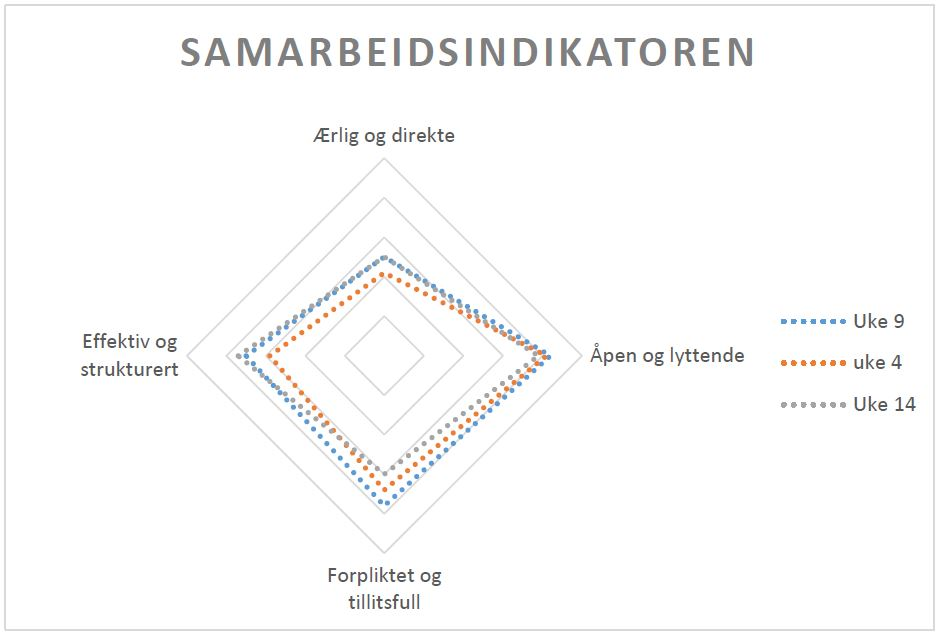
\includegraphics[scale=0.6]{images/samind2.JPG}
    \caption{Gruppas diagram fra samarbeidsindikatoren.}
    \label{fig:my_label}
\end{figure} 

\newpage

 Ut ifra hva som ble sagt i situasjonen var Håkon veldig ærlig og direkte, mer enn hva "normalen" for gruppa var. Dette kom kanskje som en respons på at Ali også hadde vært utenfor "normalen" med tanke på struktur da han gjentatte ganger hadde kommet for sent og ikke fulgt avtalen om å ikke holde på med mobilen når andre snakker. Dermed oppsto det en mismatch i samarbeidsindikatoren som kan ha ført til at situasjonen oppsto i utgangspunktet. \\

 Underveis i samtalen beklaget Håkon seg for måten han hadde ordlagt seg på og hadde forståelse for og syntes det var leit at det ble oppfattet som kjefting. I situasjonen var ikke Håkon så opptatt av hvordan budskapet skulle mottas så lenge det ble mottakeren hadde forstått budskapet og tatt dette til følge. Håkon, målbevisst som han er, var mer opptatt av å løse det underliggende "problemet", enn å tenke på hvordan det ville bli lagt fram. Ali ble på den andre siden så opprørt av tonen til Håkon at han ikke fikk med seg innholdet av det han sa, men heller måten han sa det på. Dermed handlet det for Ali heller en om hvordan han ble snakket til som person, heller enn sakens innhold.\\
 
 I forbindelse med diskusjonen om fravær nevnte Ali at nordmenn var veldig fokusert på viktigheten av å overholde avtaler som ble gjort. Dette er en observasjon flere i gruppa følte seg enig i. Anders mener at de nordiske landene generelt er mer firkantet enn resten av Europa, og verden for den del, på å være presis og å overholde avtaler. Alis lengste forsentkomming ble begrunnet med en setning som gav assosiasjoner til utsagnet \textit{"Min tid er viktigere enn din tid"}. De andres syn på forsentkomming kan gjøre at man syntes det er respektløst å ikke komme til avtalt tid, særlig hvis det skjer over flere ganger. Dermed \textit{kan} det å komme for sent tolkes som mangel av respekt for gruppas tid i fellesskap.\\
 Ali nevnte at grunnen til at han reagerte på måten han gjorde, var at han følte en mangel på respekt slik han ble snakket til. Han mente Håkon kjeftet på han og at det viser mangel på respekt.\\
 
 Begge følte da en mangel på respekt, men på forskjellige plan. Håkon fordi han følte at Ali ikke brydde seg om viktigheten med å komme tidsnok og dermed ta av fellesskapets tid, mens Ali følte en mangel av respekt fordi han følte han ble kjeftet på. \\
 
Fra kapittelet om "Valuing Diversity" i EiT-kompendiet sies det:\\

\textit{"..Bringing diverse individuals together does not result automatically in positive outcomes..."}\\{[Johnson & Johnson, 1989]}
, se \cite{EiTkomp}.\\

Her kan det tenkes at forskjellene mellom Håkon og Ali både personlig og kulturelt kan ha gjort det lettere å skape friksjoner dem imellom. Det kommer tydelig frem at de har forskjellige forventninger til adferd og respekt. Disse forventningene har gjerne forankring i kulturen man har oppvokst i.\\
 
Hvordan har disse situasjonene gitt utslag på gruppa som helhet over hele semesteret? I figur 3.1 ser vi utviklingen av samarbeidsindikatoren over tid. Det er ikke store endringer å spore men det punktet med størst variasjon er variabelen "Forpliktet og tillitsfull". Særlig ser vi at denne indikatoren har fått seg en knekk ved den siste målingen og gått ned noen poeng. Dette tror vi skyldes at tilliten innad i gruppa sank etter at denne situasjonen dukket opp, noe som er uheldig.


\newpage

\subsection{Aksjoner}


Denne hendelsen skjedde på en av landsbyens siste dager. Det ble dermed ikke diskutert så mye om hvordan vi kunne jobbe for å unngå en slik situasjon videre, siden det ikke var så mye tid igjen. Det ble generelt lagt vekt på at man skal respektere at hverandre er - og fungerer - forskjellig. At det kan være viktig å være litt varsom på- eller tenke seg om en ekstra gang før man ytrer noe.\\\\

Dersom vi skulle videreført vårt prosjektarbeid, hadde vi derimot et forslag til hvordan å takle slike situasjoner bedre i framtiden. En av øvelsene vi ble presentert for gjennom EiT, var gruppeøvelsen "2+1". Her skulle vi gi 2 positive tilbakemeldinger og 1 negativ. Dette ga trening på både å gi og få ris og ros. Det flere av gruppemedlemmene bet seg merke i, var hvor hyggelig det var å få positive tilbakemeldinger, gjerne for ting de ikke var oppmerksomme på at de gjorde. Dette ga umiddelbart god stemning i gruppa. Effekten av den negative tilbakemeldingen kunne for samtlige også regnes for å gi et positivt utfall. Alle i gruppa sa de ble oppmerksom på ting de gjerne ikke tenkte over, men flere kommenterte at det var noe de ønsket å ta tak i og jobbe videre med. Dermed ga dette en slags selvregulerende effekt på de negative egenskapene oppfattet av gruppa, og ikke minst ga en \textit{arena} for hvor det var greit å komme med negative tilbakemeldinger eller ting man ikke var fornøyd med.\\
\\
Sett i retrospekt kunne kanskje Håkon luftet på frustrasjonen sin tidligere angående hva han følte for Ali sin forsent-komming, før det bygget seg opp til et utbrudd. Ali tror også han mye bedre ville tatt i mot budskapet i kritikken, dersom det ble lagt fram i en slik arena. Ali stod veldig sterkt på at dersom man skal komme med "konstruktiv kritikk" eller si noe man er misfornøyd med om en annen person, så skal det legges fram på en nøytral og saklig måte. Her tror gruppa at en regelmessig innføring av "2+1" kunne lagt til rette for dette.


\newpage
\section{Case 2 - Anders blir oversett }

\subsection{Situasjon}

 Landsbydag 9 gikk mot slutten, og vi nærmet oss det klokkeslettet hvor vi vanligvis begynner med våre personlige refleksjoner. Det hadde blitt en del prat den siste tiden før vi skulle påbegynne refleksjonene, så atmosfæren lå til rette for fast og løst prat. En hel arbeidsdag var snart omme, så skillet mellom faglig og personlig prat ble mindre og mindre. Klokka slo 16.00 og tiden for personlig refleksjon var kommet. Gruppa hadde tidligere bestemt seg for å begynne med dagens reflektering presis klokken 16.00, for å få nok tid før vi måtte dra hjem for dagen. Jonas, Håkon og Lars diskuterte fortsatt, mens Ali satt på PCen. Det var uvisst for Anders hva Ali så på. Det er en generell tillit i gruppa som bygger på at man jobber når tiden er avsatt til jobbing. Til tross for dette hører Anders at praten til Jonas, Håkon og Lars sklir bort fra det faglige. \\

\textit{"Vi har meldt oss på, men i fjor ble vi diskvalifisert, så det er usikkert om vi får lov i år."}{--Lars}\\

Lars trekker på smilebåndet, og forteller om hvordan hockeylaget han spiller for er litt røffe i kantene. De får kanskje ikke får spille i turnering i år. Jonas og Håkon flirer. Klokka har nå bikket fem over fire og Anders tenker at dersom vi skal følge det målet vi hadde satt tidligere på dagen, så må vi komme i gang med de personlige refleksjonene våre.\\

\textit{"Gutta, nå er klokka fem over fire. Skal vi begynne med dagens personlige refleksjoner eller?"}{--Anders}\\

Blikkene fra Lars, Håkon og Jonas vrir seg mot Anders, men hodene flytter seg ikke. Det som sies blir registrert, men kroppsspråket deres anerkjenner det ikke.\\

\textit{"Jo da, sant det Anders."}{--Jonas}\\


Det går ikke mange sekundene fra Jonas sa seg enig, til samtalen er igang igjen. Håkon var fortsatt nysgjerrig på hva som skjedde med hockeylaget til Lars året før, og Jonas ville gjerne høre det samme. Øynene til Ali glir ned igjen på skjermen, da han ikke virket helt ferdig med hva han holdt på med. Denne reaksjonen fra samtlige i gruppa gjorde Anders litt irritert, og han tenkte at han skulle gjøre et lite eksperiment. Anders tok opp refleksjonsboka si og begynte å skrive, samtidig som han skulle bemerke seg hvor lang tid det ville ta fra han begynte på det avtalte arbeidet, til resten fulgte etter. Først etter fem minutter har alle gruppemedlemmene påbegynt refleksjonsskrivingen. Dette synes Anders var for dårlig, og valgte å ta det opp mot slutten av dagen.


\newpage


\subsection{Refleksjoner}

Etter å ha diskutert situasjonen i ettertid har det kommet frem forskjeller i hvordan man tolker både det som blir sagt og måten man legger fram argumentene på. Anders følte han tydelig uttrykket hva han ønsket gruppen skulle gjøre, men på en lite autoritær måte. Grunnen til at han ikke ønsket å være autoritær var fordi gruppa hadde en flat lederstruktur uten en utpekt leder. Han tror at grunnen til at beskjeden ikke ble tatt på alvor var fordi gruppa ikke kjente hverandre godt nok enda. Derfor er det vanskelig å vite hvor alvorlig et slikt ledende spørsmål blir mottatt. Selv om situasjonen oppstod halvveis ut i semesteret så mente Anders at det var for tidlig til at gruppa klarte å plukke opp signalene og væremåten til hverandre, på en måte hvor man faktisk forstod hva man mente. Gruppa kjente hverandre for dårlig til at en subtil beskjed skulle oppfattes som en "kommando". Nettopp av denne grunn ønsket ikke Anders å framstå som en autoritær type. Dette var grunnen til at han prøvde å få gruppa til å gjøre noe med kun et spørsmål.\\

Jonas og Ali følte det motsatte av Anders. De mente de kjente gruppa godt nok på dette tidspunktet til at de følte seg avslappet. Derfor trengte de ikke å følge med på slike signaler like mye som de gjorde i begynnelsen av semesteret. 
Lars satt med en oppfatning av situasjonen som en blanding av de to overnevnte. Han mente vi hadde blitt såpass kjent med hverandre at man føler seg komfortabel nok til ikke å holde fokus på å tolke signaler hele tiden, men samtidig ikke komfortabel nok til å skjære gjennom med ting. 
Det ble derfor en missforståelse i gruppa. Anders følte han hadde uttrykket seg klart og tydelig og følte seg derfor ignorert over at han ikke ble hørt mens resten av gruppa ikke hadde oppfattet situasjonen på den samme måte. \\

Denne situasjonen har fått Håkon til å tenke på hvor seriøst gruppa tar seg selv. Når gruppa mer eller mindre har blitt enige om å skrive refleksjoner klokka 16, men kollektivt bryter det løftet til fordel for uviktig prat, stiller han spørsmål ved hvor seriøst vi tok dette løftet til å begynne med. Når gruppa reflekterer rundt dette i ettertid, stiller Håkon spørsmål til akkurat hva det er som gjør at vi sier vi skal gjøre en ting, men ender opp med å gjøre noe annet. Hans tanke er at de fleste i gruppa setter det å hygge seg høyere enn jobbe med prosjektet til avtalt tid. Dette mener han strider med hva vi som gruppe har blitt enige om tidligere, og med hva hvert enkelt medlem har sagt de anser som viktig. Alle i gruppa har tidligere sagt at vi må ta det vi blir enig om å gjøre seriøst. Likevel har det dannet seg en slags kollektiv forståelse for hvordan man forholder seg til hverandre og oppgavene, som nesten alle i gruppa deler og som ikke stemmer overens med hva vi har avtalt.\\

Lars tror at vi ikke bare bryter tidligere avtaler for egen hygge. Han mener at det er svært viktig for sluttproduktet at gruppa har god kjemi og trivsel, og at det derfor skal være rom for snakk utenom det faglige. Alle sier seg enig i dette, men spørsmålet er i hvilken grad. Skal trivsel alltid trumfe arbeid, eller bare av og til? Lars trodde at det i denne situasjonen resulterte i at folk var slitne og at det var da helt vanlig menneskelig atferd å fokusere på å more seg selv i større grad. Mulighetene for frustrasjon når man er sliten er langt høyere, og tilbøyeligheten for å hygge seg er større. Dermed mener Lars at det ville være mest konstruktivt for gruppas helhetlige framgang å prioritere trivselen mot slutten av dagen. \\

Håkon kjøper ikke helt dette, og mener heller at vi bare skyr arbeid når vi er slitne og at fokuset på hygge er mer en distraksjon enn noe konstruktivt. Han tror ikke dette har videre positiv innvirkning på sluttproduktets resultat. Dette mener Lars blir litt feil, siden trivsel er en viktig nøkkel for prestasjonen vår. Anders kommenterer at dette virker som en vanskelig balansegang. Fra artikkelen "Promote an Appropriate Ratio of Task and Supportive Communications" i EiT-kompendiet \cite{groupEfficiencyModel}, sies det at de mest effektive gruppene bruker omlag 70-80\% av all sin kommunikasjon på temaer relatert til oppgaver og mål. Her brukes eksempelet om at dersom man diskuterer en fotballkamp i en lengre periode, bør man flytte fokus tilbake til arbeidet. Men, dersom det har blitt jobbet intenst i en lengre periode, bør det belønnes med litt vilkårlig løst prat for trivselens skyld. \\

Det kom fram i gruppereflektering at denne situasjonen også er litt knyttet til en annen splittelse innad i gruppa som gjelder tidsbruk. Anders syntes ikke det var poeng i å sitte til kl 17.00, bare for å sitte til kl 17.00, selv om det var dette som ble bestemt å være den faste arbeidstiden. I stedet for å sitte en halvtime og prate om sosiale ting kunne Anders heller ha tenkt seg å dra hjem. Han har nemlig fast avtale på onsdager kl 17.00 om felles middag i kollektivet han bor i. Anders har et ønske om å være hjemme til denne tiden, men føler ikke at det er en god nok grunn til å framskynde arbeidet i gruppa slik at han kommer hjem til dette tidspunktet. Han synes personlige preferanser er underordnet arbeidsavtalen gruppa har laget.\\

Dette var enda en grunn til at han prøvde å subtilt påvirke gruppa slik at gruppa blir ferdige før 17, men kun dersom det var ikke-faglig snakk. De andre gruppemedlemmene vet at Anders har denne avtalen og det har tidligere vært en diskusjon rundt dette. Der kom det fram at gruppa mente arbeidstiden var viktigere enn at han skulle rekke en middagsavtale som stridet med arbeidstiden. Anders var originalt enig i dette, og det førte da kanskje til at han ikke var like bestemt når han foreslo at vi skulle begynne refleksjonsskrivinga. Når gruppa reflekterer over dette i ettertid, kommer det fram at det var litt synd at gruppa stod så hardt på at hans middagavtaler skulle vike for arbeidstiden, når denne arbeidstiden ble brukt til uviktig snakk.
\\
%- 1) Anders følte han var tydelig i hva han ønsket at gruppa skulle gjøre, men det ble ikke oppfattet som tydelig av de andre i gruppa.

%- 1) Anders tror det kan være for tidlig til å plukke opp signalene/væremåten til hverandre. Anders ønsker ikke å skjære gjennom enda. 

%- 2) Jonas og Ali tror litt det motsatte, hvor de føler seg såppass avslappet at de ikke følger meg like sterkt på signaler fra andre.

%- 3) Lars tror det kan være et grenseskille mellom de to overnevnte situasjonene, hvor man føler seg komfortabel nok til å ikke være obs hele tiden, men ikke komfortabel nok til å skjære gjennom med ting.

%- Anders har følt seg oversett litt tidligere, og det har kanskje underbygget en følelse som boblet litt opp til denne situasjonen.

%- 4) Håkon setter spørsmål ved gruppas integritet til seg selv. Tar vi oss på alvor når vi setter en frist men ikke følger den? Anders tror vi kanskje prioriterer trivsel høyere enn framgang i prosjektet. Lars tror det er viktig å ha fokus på trivsel for å gjøre et godt prosjekt.

%- 4) Anders synes det er en vanskelig situasjon å balansere mellom å la lite viktig prat bryte mellom prosjektets planer og framgang.

%- 5) Anders synes at sin grunn (å bli ferdig for å gå hjem og spise middag) kanskje ikke var viktig nok for å presse på.

%- 5) Anders synes at det ikke er noe vits i å sitte til 17 bare for å sitte til 17.

%- 6) Hvordan pushe folk til å jobbe uten å framstå kjip?


\newpage

\subsection{Aksjoner}

I starten av dette faget, rundt tiden vi dannet vår samarbeidskontrakt, så ble gruppa enig i at når noen snakker så skal man legge fra seg alt annet og følge med. Man skulle følge såpass med at man tok til seg det som ble sagt og skulle kunne svare konstruktivt på det, dersom man hadde innspill. Når forslaget til Anders om å starte dagens personlige refleksjonsskriving så vidt blir anerkjent, kan det tyde på at her innfridde ikke resten av gruppa godt nok på dette punktet. Det er vanskelig å innordne seg til slik man avtaler at man skal oppføre seg. Dette gjelder spesielt når man begynner å bli sliten i hodet etter en lang dag. Likevel er det et punkt gruppa mener er svært viktig for at alle skal føle seg inkludert, og ser dermed på dette som noe som bør jobbes kontinuerlig med å etterstrebe så bra man klarer.\\
\\

Under landsbydag 3 hadde vi en øvelse som het "ta plass, gi plass", der vi skulle visualisere hvor stor andel av taletiden og hvor stor del av rommet vi mente at hvert medlem tok. Det viste seg at alle i gruppa hadde omtrent det samme bilde på hvor mye plass hver enkelt tok. Det så omtrent ut som Figur \ref{fig:taplass}.

\begin{figure}[H] 
    \centering
    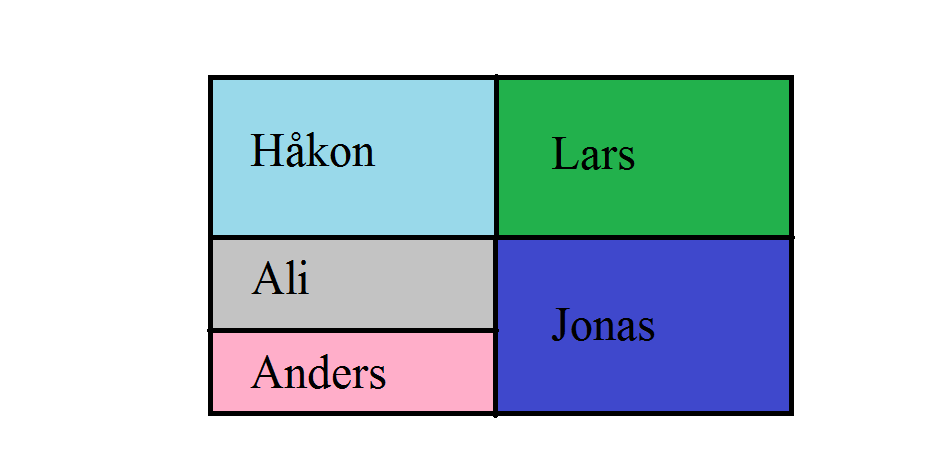
\includegraphics[scale=0.5]{images/taplass.png}
    \caption{Visuell framstilling av hvor mye plass hvert gruppemedlem tok}
    \label{fig:taplass}
\end{figure}\\


Ali og Anders tok ikke ordet like mye i starten. Når gruppa reflekterte rundt dette kom det fram at Anders var litt usikker på om hva han hadde å si var viktig nok til at det var behov for å si det. Det ble spekulert i om Anders ikke følte seg komfortabel nok med å si fra sterkt nok om hva han mener, i frykt for å si "noe dumt". Dette trodde Anders at kanskje resulterte i at han ufarliggjorde det han sa, og at gruppa kanskje ikke tok det like seriøst. Her mente Anders at et virkemiddel for å ikke bli oversett på det han sier, er at han må å være mer frampå og ta mer plass. På denne måten vil det minske risikoen for at hva han sier ikke blir anerkjent, og at Anders vil føle seg mer delaktig i bestemmelsene. Det vi i gruppa kom fram til at vil være en optimal balansegang for oss, er at personen som snakker må prøve å være bestemt i å få fram synspunktet sitt. Resten av gruppa må ha i bakhodet at det er viktig å være attentativ og respekterende ovenfor den som snakker for at alle skal føle seg komfortable og inkludert i gruppearbeidet.\\
\\

%- ta plass gi plass

%- de som tar mye plass er kanskje litt mer hensynsløs i snakkestilen.

%- sette fast klokkeslett og være mer obs på det.

%- Anders må tørre å være litt mer standhaftig (faglig innhold)

%- Andre må være litt mer obs

\newpage
\section{Case 3 - Reaksjon på arbeidsfordeling}

\subsection*{Situasjon}
Det er den 7. landsbydagen og alt ligger til rette for at dagen i dag skal brukes til konstruktivt arbeid. I ukene i forveien har det blitt lagt vekt på å bli kjent med hverandre, kartlegge våre ambisjoner for prosjektet samt bli enige om konsept vi skal jobbe med i ukene framover. Disse ukene har vært greie, men nå er tålmodigheten vår tøyd et stykke og alle ser fram til å begynne ordentlig på prosjektet. Dessverre er ikke gruppa fulltallig, da Ali er fraværende på grunn av sykdom.\\
\\Da vi bestemte oss for konseptet vi skulle arbeide med, ble det foreslått av veileder at vi i tillegg til en prototype også skulle se på hva slags samfunnsrelaterte oppgaver og utfordringer som måtte løses for at Truck Platooning skulle bli en realitet i framtiden. Dette syntes vi hørtes fornuftig ut og gruppa ble derfor delt i to subgrupper. Tre medlemmer av gruppa skulle konsentrere seg om prototype-utvikling, mens de to andre skulle konsentrere seg om de samfunnsrelaterte utfordringene. 
\\Ettersom vi var en ganske todelt gruppe med tanke på bakgrunnene våre, falt arbeidsfordelingen seg ganske naturlig. Håkon og Lars skulle ha hovedansvaret for prototyping, da denne arbeidsoppgaven krever innsikt og erfaring i programmering og datateknologi. Dette passet de veldig bra, ettersom de studerer kybernetikk og elektronikk. Ali skulle bistå  begge sub-gruppene da han også er fra kybernetikk, men hadde interesse for begge temaene. Den andre subgruppa består da av Jonas og Anders som begge kommer fra maskin-linja.\\

\\Det kan spores noe missnøye eller skuffelse hos noen av medlemmene angående denne arbeidsinndelingen. Jonas valgte denne landsbyen siden han er interessert i data og IT og ønsket å jobbe innen dette fagfeltet i dette prosjektet. Jonas er derfor litt skuffa når han innser at det blir mer samfunnsrelatert arbeid som skal gjøres, og ikke så mye av det tekniske han kommer til å jobbe med i dette prosjektet. Da denne arbeidsfordelingen blir bestemt, ca en uke før denne landsbydagen, sier Jonas ifra om dette. Men, han svelger kamelen da han er enig i at det bør være en samfunnsdel av prosjektet, og den mest naturlige inndelingen er at Håkon, Ali og Lars jobber med prototypen. Han ytrer at han har erfaring fra å lage prototyper tidligere i utdanningen, men innser at mangelen på IT- og elektronikkforståelse begrenser ham her.\\
\\
Ettersom vi er to grupper som holder på med vidt forskjellige deler av samme prosjekt ble det foreslått av Håkon den foregående uken at vi bruker programmet Trello, se appendiks B. Dette er et organiseringsverktøy som muliggjør bruk av SCRUM-modellen, slik at vi alle har oversikten over hva hver enkelt jobber med. Tanken bak dette er å gjøre det oversiktlig for alle å se hva hverandre holder på med. Uken før  gikk dermed til å bestemme spesifikke arbeidsoppgaver og fylle de inn i Trello, slik at vi denne uka kunne begynne å jobbe med de.\\

\\Etter dagens innsjekk påbegynnes arbeidet med oppgavene vi bestemte oss for uken før. Det senker seg en ro blant gruppa da alle er fokusert på å vise at vi kan holde ord og løse de oppgavene vi er satt til å gjøre. Det blir stille da arbeidet starter. Jonas sitter med musikk på øret og leser seg opp på statistisk sikkerhet, Anders er dypt konsentrert av å forstå hvilke parametere som bidrar til luftmotstand, Ali gjør research på European Truck Platoon Challange, Håkon leser seg opp på Nordic Semiconducter sin chip, mens Lars ser etter løsninger for hvordan vi skal svinge og styre prototypen. 
Rett før lunsj kommer fasilitator Martine med en bemerkning; \\

\textit{"Dere må slutte å være så stille. Det mye morsommere å fasilitere når dere ikke jobber så hardt."}{--Martine}\\ 

Etter lunsj fortsetter vi der vi slapp og går til hvert vårt arbeid. Anders bemerker seg at det er veldig lite kommunikasjon innad i gruppa, men tenker at det er naturlig ettersom vi holder på med vidt forskjellige ting. Jonas ser opp fra skjermen og kommer med en snodig bemerkning om hvor langt en flåte med autonome biler må kjøre før man med sikkerhet kan si at det er like sikkert som en vanlig sjåfør. Gjennom dagen kommer det noen få slike bemerkninger, men ellers er det veldig stille da alle er tilfreds med arbeidet vi gjør hver for oss. Da det nærmer seg slutten av dagen er det tid for gruppe-refleksjon. Under gruppe-refleksjonen forteller vi litt om hva hver enkelt har jobbet med i løpet av dagen, men samtlige av oss kommer med den samme observasjonen. Det har vært veldig stille i dag.\\ 

\textit{"Jeg synes det er godt å få begynne å jobbe. Få jobbet i fred og ro. Det har vært lite diskusjoner, men for lite informasjonsflyt. Rart å jobbe i en slik setting igjen, tror det er viktig med dialog fremover slik at vi blir mer involvert i arbeidet til hverandre."}{--Håkon}\\

\textit{"Synes i grunn det var litt godt å møte opp for så å bare starte. Det har vært veldig effektivt og jeg føler jeg har fått utrettet mye mer i dag enn tidligere. Likevel har det kanskje ikke vært så mye involvering fra hverandre, og jeg er litt usikker på hva de andre har gjort så langt. Bør vi ha steg i løpet av dagen der man deler hva man har gjort?. Dette tror jeg vil føre til mer involvering, uten at det går for mye ut over effektiviteten."}{--Jonas}\\

\textit{"Jeg synes også det har vært en effektiv dag, men ikke for lite involvering. Dere har fortalt hva dere holder på med, og kommet med små kommentarer fra deres oppgaver underveis. Dette har gitt meg et ganske godt inntrykk av hva som skjer på tvers av gruppa i alle fall.}{--Lars}\\
\\
Det er altså blandede følelser om hvordan vi føler arbeidsdagen har gått. På den ene siden har det vært godt å komme i gang og fått gjort noe, mens på den andre siden har det vært lite involvering og lite kommunikasjon på tvers av gruppa. Vi har en omtrentlig situasjonsoversikt men med den manglende kommunikasjonen er det fare for at vi går glipp av verdifull input som kan løfte oppgaven betraktelig.\\



\subsection{Refleksjoner}


I ettertid har gruppa reflektert over utslaget denne arbeidsfordelingen har gitt, både i forhold til gruppedynamikk men også i forhold til resultatet. Med det klare skillet mellom de to subgruppene har en god sammenføyning av prosjektene vært vanskelig. Vi har ikke opplevd det som problematisk i forhold til å få et godt ferdig produkt. Subgruppene internt har samarbeidet godt og jobbet målrettet. Derimot har behovet for samarbeid mellom subgruppene vært tilnærmet fraværende da de respektive gruppenes arbeid ikke har hatt direkte innvirkning på den andres.\\ 

En viktig del av dette faget er å erfare hvordan det er å jobbe sammen til tross for ulike av bakgrunner, erfaringer og oppgaver. Ved ikke å jobbe så tett sammen har vi redusert muligheten for å lære mer om hverandres fagfelt, men vi samtidig har vi utnyttet gruppas kompetanse på en mest mulig effektiv måte. Dette for å få fremdrift i prosjektet. Ved å ikke bruke tid på å lære opp hverandre har vi kunnet bruke tiden effektivt under de forutsetninger hvert enkelt gruppemedlem har.\\

Grunnen til at vi valgte denne arbeidsfordeling var at både Anders og Jonas følte de måtte ha investert masse tid i å lære det grunnleggende IT- og elektronikktekniske før de kunne startet med selve prototypearbeidet. Dette hadde kostet masse tid, og når selve prototypen ikke direkte er med i vurderingen av prosjektet i sin helhet, hadde dette vært mye tid investert i noe som ikke nødvendigvis hadde høynet kvaliteten på rapporten. Ali havnet midt mellom og har vært inn og ut av begge subgruppene gjennom semesteret. Han har gjort mye research og lært mye, men utbyttet av arbeidet føler han ikke har vært så stort. Han stiller spørsmål til hvor nyttig denne researchen har vært i forhold til den endelige rapporten.\\

Håkon kom med en interessant refleksjon som gikk ut på at det er sluttproduktet vi har fokusert på, ikke å dra mest mulig lærdom av hverandres fagkomptanse. Dette var gruppa enige i. Det er tross alt sluttproduktet vi skal vurderes etter, ikke direkte hvordan vi har kommet fram til målet. Dermed kan man rettferdiggjøre arbeidsfordelingen ved å hevde at det var den mest effektive måten å nå målet på, men med tanke på læringsutbytte til hver enkelt student så var det kanskje ikke den beste fordelingen for å lære av hverandre. \\

En ting vi følte kunne være en ulempe, var at vi ikke stilte nok kritiske spørsmål til hverandre. De to subgruppene hadde tillit til hverandres arbeid og antok at det de andre holdt på med eller kom fram til var nyttig for prosjektet som helhet. Her antar Håkon at dersom vi hadde jobbet mer med det samme, eller i det minste vært mer inkludert i hverandres arbeid, så kunne vi presset hverandre på akkurat \textbf{hvorfor} vi gjorde som vi gjorde. Dette mente Håkon kunne styrket produktene fra hver enkelt subgruppe. For sluttproduktet tenkte Anders på dette positivt. Som mer eller mindre utenforstående for hva de andre gjorde, ga det samme innblikket i stoffet som for noen som leser det for første gang. Dermed når det kom til rapportskriving, kunne man be vedkommende utdype eller reformulere seg slik at innholdet enklere forståes. Dette førte til flere kritiske spørsmål og en rekke omformuleringer når rapportene skulle gjennomgåes før levering.\\

Ved å ikke ha et eierforhold til innholdet er derimot terskelen høyere for å skjære igjennom med store endringer da en ikke kjenner sammenhengen på samme måte som forfatterene. Det samme gjelder arbeidet med prototypen. Uten å ha kjennskap til hvordan de ulike modulene fungerer er det vanskelig å komme med konstruktive tilbakemeldinger og forslag.\\

Ali mente at det ble lite eierfølelse til prosjektet som helhet, når man jobbet med så forskjellige temaer. Det var rimelig effektivt å dele opp gruppen på denne måten, men han følte at det ble gjort nærmest som to separate prosjekt. Lars sa seg enig i dette, og innrømte at han ikke visste mye om hva som hadde blitt gjort på samfunnsdelen av prosjektet. Dette syns Lars var synd, da mye av poenget med EiT var å jobbe sammen. Lars reflekterte rundt dersom vi skulle startet på nytt i dag, kunne vi gjort det annerledes. Han trodde det kunne blitt mer samarbeid dersom vi delte opp de to oppgavene våre i to bolker. Først hadde vi gjort research på Truck Pooling og ferdigstilt alt på samfunnsdelen sammen. Etter dette kunne vi utviklet prototypen i felleskap. Dette var en interessant idé som blir drøftet litt nærmere som en av aksjonene vi kunne tatt.\\

Det at gruppa har fordelt arbeidsoppgavene på denne måten har ført til mangel på samhørighet i gruppa. Dette er ugunstig da samhørighet har en rekke positive effekter innad i en gruppe, se \cite{Promotegroup}:
\begin{itemize}
    \item [-] Økt konformitet.
    \item [-] Økt gruppeinflytelse over øvrige medlemmer.
    \item [-] Hvert medlem er mer fornøyd/tilfreds med gruppa.
    \item [-] Bedre samarbeid.
\end{itemize}

En ikke-sammensveiset gruppe er i faresonen for å ta dårlige avgjørelser. I kompendiet blir dette kalt \textit{groupthink}. Dette kjennetegnes ved\cite{EffectiveTeams}:
\begin{itemize}
    \item [-] Når grupper med hensikt jobber i isolasjon og ikke deler funn eller konklusjoner med andre utenfor gruppa. Da øker sjansen for å ta dårlige avgjørelser.
    \item [-] Hvis gruppelederen kontrollerer diskusjonen og uttrykker sine meninger helt fra starten av.
    \item [-] Hvis gruppa står ovenfor en viktig eller stressende avgjørelse øker tendensen for å ta en rask avgjørelse i den hensikt å redusere stresset. Dette igjen resulterer ofte i at en dårlig avgjørelse blir tatt.
\end{itemize}

Arbeidsfordelingen var ikke en dårlig avgjørelse, men sett i lys av hvordan gruppedynamikken fungerte i ettertid kan det hende gruppa har mistet noen av de positive sidene ved gruppesamarbeid. Vi ser at subgruppene kan kjennetegnes ved det første kriteriet for \textit{groupthink}. Dette blir selvsagt hypotetisk og spekulativt, men kanskje verdt å ta til ettertanke.
\newpage

\subsection{Aksjoner}
For å bedre kommunikasjon, samspill, gruppedynamikk og eierskap til prosjektet innførte gruppa daglige briefinger. Briefingene ble gjort etter innsjekk, før lunsj, en gang mellom lunsj og refleksjoner samt på slutten av dagen før refleksjonene. Alt i alt, fire daglige briefinger. Den første briefingen besto som regel av å informere om hva man tenkte å bruke dagen på, hvilke tema, hvilke deloppgaver osv. Det var lagt opp til at man her skulle få input fra de andre gruppemedlemene og diskutere hva som var viktig å få gjort samt å avgjøre om hva man skulle legge mest vekt på. De andre briefingene var korte statusoppdateringer hvor resten av gruppa fikk inntrykk av hvordan det hadde gått samt progresjonen på alle oppgavene.\\

På denne måten var det enklere for alle medlemmene å skaffe seg en oversikt over hva som skjedde og konkrete utfordringer i hver oppgave. I tillegg fikk alle en bredere samhørighet og eierskap til prosjektet og gruppa følte at dette var et positivt og nødvendig tiltak både i forhold til prosjektet, men også det sosiale. Disse briefingene tok omtrent 40-50 miunutter av arbeidsdagen men resultatet var en felles forståelse av hvordan gruppa lå an totalt sett. Gruppa følte at dette var et positivt tiltak som resulterte i progresjon.\\

En annen aksjon gruppa gjorde var å benytte SCRUM metodikken. Det innebærer blant annet de tidligere nevnte briefingmøtene. For følge opp SCRUM valgte vi å bruke verktøyet Trello. Dette er et verktøy som viser status på prosjektet som beskrevet ovenfor. Ved å bruke dette verktøyet aktivt og holde det oppdatert kunne gruppemedlemmene alltid holde seg oppdatert over status og hva de andre medlemmene holdt på med. Dette gav likevel ikke et komplett, helhetlig bilde, men hjalp gruppemedlemmene i å være oppdaterte på hva den andre subggruppen brukte tiden på.\\





%Consensus side 62/63, ikke 100\% av gruppa trenger å være enige, men 70-80\%. 
%Effektiv metode for problemløsning: Shaw: 
%1.	erkjenne at det er et problem
%2.	diagnosisere problemet
%3.	ta en avgjørelse
%4.	akseptere og implementere avgjørelsen
%alternativt:
%1.	orienteringsfase
%2.	diskusjonsfase
%3.	avgjørelsesfase
%4.	implementeringsfase
%«hvis medlemmene ikke føler de kan bidra fritt med ideene, det vil bli vanskligere for gruppa å lykkes.» s64
%S65: diversity norms: medlemmer er forventet å komme en time før. Normer som dette kan hindre individuell frihet og forårsake «resentment»/avsky. 
\chapter{Medlemserfaringer}


\section{Lars sine 3 hovederfaringer}

\subsubsection*{Erfaring 1 - Sosiale aktiviteter tidlig i prosjekter er viktig}
I starten av arbeidet med Eksperter i Team var det mye fokus på å bli kjent gjennom ulike sosiale leker og øvelser.
For meg som ikke var vant til slik, slo det meg som litt underlig at vi skulle bruke såpass mye tid på aktiviteter som ikke virket innlysende å ha innvirkning på selve prosjektet der og da.
I retrospekt ser jeg verdien av dette. Det er mye lettere å starte arbeidet med prosjektet når alle er litt kjent og du har en idé om hva andre tenker og finner interessant.
Det er mulig jeg ikke har tenkt over dette før, siden jeg i alle tidligere prosjektarbeid har kjent de jeg har arbeidet med. Til senere prosjekter i arbeidslivet ser jeg verdien av dette, da det er sjeldent du kjenner alle du vil jobbe i et prosjekt med. 

\subsubsection*{Erfaring 2 - Gjensidig respekt for tanker og idéer er viktig}
Vi fant tidlig ut at noen av gruppemedlemmene snakker mer og skyter inn flere kommentarer enn andre, inkludert meg selv. På bakgrunn av dette ble vi enige om å la folk snakke ut og få fullføre resonnementene sine uten å bli avbrutt. Gjennom å fokusere på dette gjennom prosjektperioden føler jeg diskusjonene har hatt god kvalitet og at alle føler de har blitt hørt.
De aller fleste argumenter for og imot ulike avgjørelser har blitt presentert på en god og sammenhengende måte, siden man har fått tid og plattform til dette.
Ved å fokusere på dette har jeg blitt mer bevist på helheten av andres argumentasjon.
Jeg tror dette førte til at flere riktige beslutninger ble tatt og at prosjektarbeidet ble lettere.

\subsubsection*{Erfaring 3 - Refleksjoner gir prosjektet bedre fremdrift}
Hele idéen med refleksjonsarbeid var nytt for meg og noe jeg anså som unødvendig i starten. 
Etter at gruppa ble mer sammensveiset ble også refleksjonsarbeidet bedre. Gjennom å ta opp ulike situasjoner gjennom dagen fikk vi diskutert og lagt frem alle sine syn. 
Dette førte igjen til at vi tok flere avgjørelser som bedret prosjektarbeidet og fremdriften i prosjektet.
Gjennom refleksjonene ble vi blant annet enig om å ha korte oppdateringsmøter gjennom dagen. Dette sikret at alle arbeider med noe som bidrar til sluttproduktet. Alle gruppas medlemmer fikk også et større eierskap til hele prosjektet, ikke bare til den delen de arbeidet med.

\section{Anders sine 3 hovederfaringer}

\subsubsection*{Erfaring 1 - Refleksjon kan gi andre forutsetninger}

I motsetning til andre prosjekter hvor det har vært resultatet som har stått i fokus, har det i dette tilfellet vært veien til resultatet som vi skal lære av og fokusere på. Det har vært en annerledes tilnærming til å gjøre et prosjekt, og effektiviteten i prosjektet har ikke vært like høyt for hva som er vanlig for meg, men læringsutbytte har vært større. Selv om læringsutbytte har vært like teknisk som det vanligvis bruker, har læringen vært om meg selv. Hvordan \textit{jeg} fungerer i en gruppe og om hvordan forskjellige faktorer påvirker gruppedynamikken og hvordan gruppedynamikken påvirker arbeidet.

\subsubsection*{Erfaring 2 - Kartlegging kan være produktivt}

I starten av faget brukte vi lang tid på å bli kjent og bestemme oss for hva vi skulle velge som tema. Av erfaring er dette noe som tar lang tid og det er ofte usikkert om man har valgt et godt tema før man faktisk har startet på arbeidet. Vi brukte mye tid i starten på å kartlegge hva vi ønsket å gjøre og hvilke temaer som vi skulle fokusere på. Det at vi brukte tid på dette i starten tror jeg sparte oss for mye tid senere i prosjektet. Etter å ha gjort noe researh kunne gruppa finne hvilken retning vi skulle vinkle arbeidet. Dermed ble det enklere å utelukke punkter som ikke fulgte hovedprofilen, og prioriteringen av hva som var viktig ble enklere. 

\subsubsection*{Erfaring 3 - En munn, to ører}

Fra starten av fastslo vi at vi skulle la hverandre prate ferdig og ikke avbryte hverandre når vi diskuterte. Jeg har personlig tatt dette veldig seriøst og jeg tror ikke jeg har avbrutt noen en eneste gang. Dette har både en positiv og en negativ effekt. Man får presentere det man skulle si i sin helhet, uten påvirkning fra de andre, noe som virket som en fordel for de fleste. Men i løpet av prosjektet har jeg merket at jeg ikke er så god til å ordlegge meg, og at jeg kan ha godt av å få innputt til det jeg snakker om. Likevel mener jeg at man kan komme lengre som gruppe ved å ha tålmodigheten til å høre på andre framfor å avbryte å komme til en beslutning. Det er en grunn til at vi har to ører, men bare en munn.

\section{Ali sine 3 hovederfaringer}

\subsubsection*{Erfaring 1 –  Hvordan gi og få tilbakemeldinger} 
 Dette faget har tvunget oss til å tenke mer på kommunikasjon. Hvordan man kan gi tilbakemelding på riktig og effektiv måte? Dette for at det skal bli tatt imot på en saklig måte, heller enn personlig. Dette er noe jeg føler jeg har fått god innføringen i gjennom semesteret og virkelig kan nå se nytten av. Sent i semesteret hadde vi en øvelse som het 2+1, en øvelse  jeg likte veldig godt. Jeg synes  det var en smart måte å gi tilbakemeldinger på. 
 
\subsubsection*{Erfaring 2 – Det sosiale betyr mye for kvaliteten av arbeid}
Noe jeg skal ta med meg videre og har fått en større forståelse for er betydningen av å ha tid til å bli kjent med hverandres bakgrunn og hvem de er som en person. Det er mange ting jeg har visst jeg ikke var god i, og kommunikasjon mellom de andre har hjulpet meg å kartlegge det og bli mer kjent med meg selv og hvordan jeg oppfører meg i en gruppe. Dette er noe jeg hadde ikke forventet når jeg meldte meg for faget. Man slutter aldri å lære om seg selv eller andre. 
 
 
\subsubsection*{Erfaring 3 - Kommunikasjon og plattform for å organisere arbeid}
I den tidlige fasen av prosjektet ble det foreslått av Håkon å bruke en arbeidsmetodikk som heter SCRUM. Jeg synes denne arbeidsmetodikken har et stort potensiale hvis den er implementert og tatt i bruk på riktig måte. Arbeidsmetodikken kan gi prosjektets fremdrift høy kvalitet, og kommunikasjon og oversikt står sentralt. Når vi møtte opp på starten av landsbydagene diskuterte vi hva som har blitt gjort siden sist, hva vi vil jobbe med videre, og om er det noen hindringer i vegen. Det å ha all informasjon om arbeidsoppgaver tilgjengelig på et sted og å tildele ansvar til enkeltmedlemmer minker sjansen for misforståelse og gir en fin arbeidsflyt utover prosjektet. 

\section{Håkon sine 3 hovederfaringer}

\subsubsection*{Erfaring 1 - Prosjektarbeid uten eierfølelse}
I dette prosjektet har gruppa jobbet veldig adskilt hva angår prototypearbeidet mot rapportskring og utforsking av temaet Truck Platooning. Jeg erfarte at før vi startet med kortere møter hvor vi kartlegger hva vi holder på med og skal gjøre utover dagen, hadde jeg ikke noe forhold til hva de rundt meg arbeidet med. Det ga en følelse av særs lite eierforhold til de ordene og tankene som ble skrevet ned i rapporten og gjorde at motivasjonen min for å opprettholde gruppesamholdet minket. Etter vi startet med kortere møter to ganger daglig for å kartlegge arbeidet vi holder på med og fortsetter med utover dagen stiger motivasjonen betraktelig. Det er godt å høre og se at de andre også jobber og holder en fin fremdrift. Derimot eierfølelsen slet jeg fortsatt med å finne da jeg aldri helt tok meg tid til å lese gjennom og prosessere og bearbeide tankene mine rundt det arbeidet de andre hadde gjort. Jeg tar med meg videre å forsøke å investere mer tid i andres arbeid for å kunne opparbeide meg et større eierforhold til prosjektet og produktet, og holde å meg oppdatert på de delene av prosjektet jeg ikke arbeider med.  

\subsubsection*{Erfaring 2 - Folkeskikk, oppmøte til avtalt tid}
Jeg har erfart at lengden av min egen lunte er kortere enn andres når det kommer til hva jeg ser på som folkeskikk, mot hva andre ser på som ikke fult så farlig. Jeg tenker på å møte opp til avtalt tid. I gruppa har det variert mye hvor gode vi har vært til å møte opp til avtalt tid. Jeg står fast på at det er folkeskikk å møte opp til avtalt tid, hvor andre har åpentbart hatt et annet syn på det. Derfor har jeg erfart hvordan jeg selv håndterer og forholder meg til personer som gjentatte ganger kommer for sent, og hvordan jeg må forholde meg til andres synspunkter. 

\subsubsection*{Erfaring 3 - Å ikke bryte inn}
Jeg liker måten vi har blitt enige om å diskutere på. Det gir meg en veldig ro når jeg får lytte til resonnementer som blir fullført, og jeg får selv si hva jeg ønsker å uten å bli avbrutt. Det fører til at det blir mindre opphete diskusjoner i gruppa. Jeg tror det gir rom for å forstå hverandre bedre når man lar folk bli ferdige, enn å skulle la de mest rappkjeftete bryte inn og ta over og styre diskusjonene i sine bestemte retninger.  
\section{Jonas sine 3 hovederfaringer}

\subsubsection*{Erfaring 1 - Åpenhet og ærlighet varer lengst}

I tidligere prosjekter har jeg latt uenigheter forbli innvendig, siden jeg har tenkt at det ikke er lenge igjen av prosjektet og la oss bare ha det fint. En ting jeg har lært gjennom EiT er at det ofte er bedre å lufte det man har på hjertet så kan man ha en diskusjon rundt det og evt. komme til en løsning. Dersom man likevel ikke har kommet til en løsning, merker jeg man føler seg bedre av å bare si hva man føler. Alle trenger ikke nødvendigvis å være enig, bare man føler seg forstått.

\subsubsection*{Erfaring 2 - Folk er forskjellige}

Etter den lille krangelen mellom Håkon og Ali så jeg to ganske forskjellige reaksjoner til en situasjon, som jeg følte jeg ville reagert på en helt annen måte igjen. Dette ga meg innsyn i at folk virkelig er satt sammen forskjellig, og at det ofte kan være lurt å ha i bakhodet når man snakker eller samarbeider med andre.

\subsubsection*{Erfaring 3 - Å ikke bryte inn}

Tidlig i EiT, når vi skapte samarbeidsavtalen, ble vi enig at når noen snakket så skulle de få snakke ferdig uten at noen skulle bryte inn. Med dette løftet virker det som alle parter \textit{hører} mer etter, og analyserer og tenker gjennom hva som blir lagt fram før man hopper på med et svar. For min del ga det også rom for å tenke \textit{hvorfor} jeg ville svare som jeg svarte, og dermed få en liten ekstra dimensjon i å bedømme om det jeg kom med var bra eller ei. 

\chapter{Grupperfaringer}


\section{Gruppeerfaring 1 - Adskilt arbeid}

Etter gruppa hadde valgt arbeidsoppgave, ble det avgjort at vi skulle gjøre litt forskjellige arbeidsoppgaver grunnet vår forskjellige bakgrunn. Det ble fort enighet om at de med elektro-bakgrunn skulle jobbe med prototypen og de fra maskin tok på seg jobben med det samfunnsmessige aspektet. Da prosjektet gikk mot slutten innså vi at ved å arbeid separert på denne måten, hadde vi lite peiling og kontroll over hva de andre holdt på med. Dette gjorde også at det ikke ble like mye gruppearbeid, men mer individuelt arbeid innad i en gruppe.

\section{Gruppeerfaring 2 - Arbeidsmetodikk}

Da vi startet å arbeide med selve prosjektarbeidet holdt vi på med flere forskjellige deloppgaver samtidig. Siden vi ikke hadde en overordnet leder, da dette gikk på rundgang, var det viktig for hvert enkelt medlem å ha en oversikt over hva gruppa holdt på med. Det var viktig å ha en overordnet forståelse av hvordan fremgangen til gruppa var. Derfor brukte vi Trello. Det er et verktøy som egner seg godt til å gjennomføre arbeidsmetodikken SCRUM. På denne måten hadde vi en oversikt over status og fremtidige oppgaver. Dette fungerte godt i starten av prosjektet, men etter noen uker ble ikke oppgaver oppdatert og metodikken ikke fulgt godt nok. Dette førte til at gruppas oversikt over fremgang og arbeid ikke ble så god som ønskelig. Erfaringen vår er at metodikken er veldig god i teorien, men krever innsats for å fungere. Det gjør at den i praksis er vanskelig å bruke. Vi erfarte hvor vanskelig oversikt i team-arbeid kan være.

\section{Gruppeerfaring 3 - Ingen avbrytelser}

Som de personlige refleksjonene bærer preg av har vi innad i gruppa vært fokusert på å gi plass til hverandre og være obs på å ikke avbryte hverandre. Vi tar fram dette som en av hovederfaringene fra dette semesteret. Det har vært ett nytt fokusområde for alle medlemmene, og det har til tider vært krevende å holde tanker inne og vente til man ikke avbryter medlemmet som snakker. Men erfaringene fra medlemmene er positive til denne regelen/loven som vi ble enige om i samarbeidskontrakten den første landsbydagen. 
\newpage
\pagenumbering{gobble}
\begin{appendices}
\pagenumbering{Roman}
\setcounter{page}{1}


\chapter{Samarbeidskontrakt}
\begin{figure}[h]
    \centering
    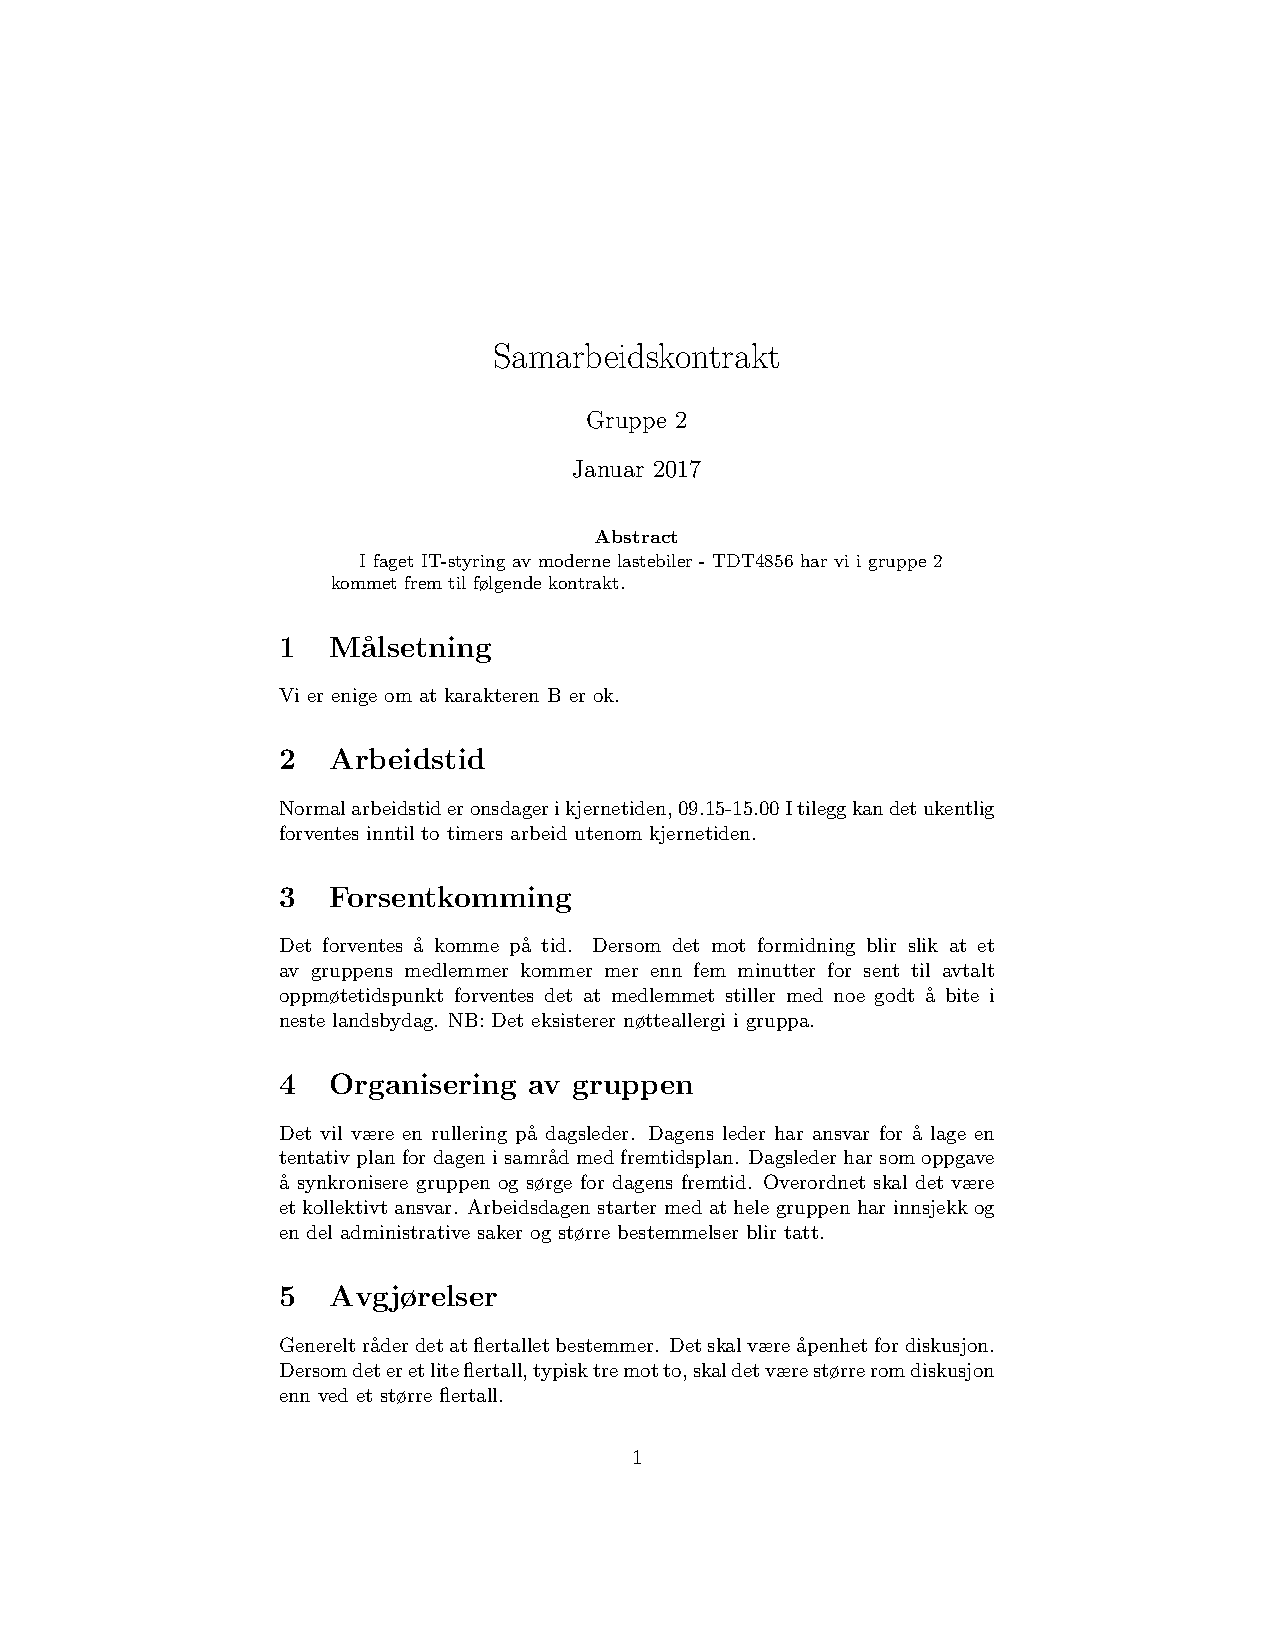
\includepdf{vedlegg/Samarbeidskontrakt.pdf}
    \label{vedlegg:Samarbeidskontrakt}
\end{figure}



\chapter{Trello}

\begin{figure}[h]
    \centering
    \includepdf{vedlegg/Trello1.pdf}
    \label{vedlegg:Trello}
\end{figure}



\end{appendices}



\newpage
\pagenumbering{gobble}

% Bibliography - edit references.bib and use the \cite command in text
\bibliographystyle{plain}
\bibliography{references}
\end{document}

